\documentclass{report}

% Packages for images.
\usepackage{graphicx}
\usepackage{float}

% Packages for mathematical formulae/symbols.
\usepackage{amsmath}
\usepackage{amssymb}
\usepackage{amsfonts}

% Packages for code snippets and algorithms.
\usepackage{listings}
\usepackage{xcolor}
\definecolor{codegreen}{RGB}{0,128,0}
\definecolor{codegray}{RGB}{110,110,110}
\definecolor{codepurple}{RGB}{163,21,21}
\definecolor{codeblue}{RGB}{0,0,180}
\definecolor{backwhite}{RGB}{255,255,255}
\definecolor{backcolour}{RGB}{248,248,248}
\lstdefinestyle{mypython}{
    language=Python,
    backgroundcolor=\color{backwhite},
    basicstyle=\ttfamily\small,
    keywordstyle=\color{codeblue}\bfseries,
    commentstyle=\color{codegreen}\itshape,
    stringstyle=\color{codepurple},
    numberstyle=\tiny\color{codegray},
    numbers=left,
    numbersep=8pt,
    frame=single,
    rulecolor=\color{black!20},
    breaklines=true,
    showstringspaces=false,
    tabsize=4,
    keepspaces=true
}
\lstset{style=mypython}
\usepackage[ruled,vlined]{algorithm2e}

% Creating the Example and Proof boxes.
\definecolor{exampleback}{RGB}{240, 248, 240}
\definecolor{exampleframe}{RGB}{34, 112, 62}
\definecolor{proofback}{RGB}{240, 244, 250}
\definecolor{proofframe}{RGB}{25, 80, 150}
\usepackage[most]{tcolorbox}
\tcbuselibrary{listings}
\newtcolorbox{examplebox}[1][]{
    colback=exampleback,
    colframe=exampleframe,
    coltitle=white,
    fonttitle=\bfseries,
    title={Example\ifblank{#1}{}{: #1}},
    arc=2pt,
    boxrule=1pt
}
\newtcolorbox{proofbox}[1][]{
    colback=proofback,
    colframe=proofframe,
    coltitle=white,
    fonttitle=\bfseries,
    title={Proof: #1},
    arc=2pt,
    boxrule=1pt
}

% Packages for styling and layout.
\usepackage{booktabs}
\usepackage{array}
\usepackage{geometry}
\usepackage{hyperref}

% Packages for plotting graphs.
\usepackage{tikz}
\usepackage{pgfplots}
\pgfplotsset{compat=1.18}

% Packages for compilation.
\usepackage{microtype}

\begin{document}

\begin{titlepage}
    \centering
    \vspace*{2cm}
    
    % Subject Title.
    {\Huge \bfseries Fundamentals of Data Science \par}
    \vspace{1.5cm}
    
    % Master's Degree and Faculty.
    {\Large Master's Degree in Data Science, Sapienza Università di Roma \par}
    {\large Faculty of Information Engineering, Informatics and Statistics \par}
    \vspace{0.5cm}
    
    % Department.
    {\large Department of Computer Science \par}
    \vspace{3cm}
    
    % Author.
    {\Large \textbf{Author:} Gianmaria Romano \par}
    \vspace{3cm}

    % Reference Bibliography
    {\Large Reference Bibliography \par}
    {\large M. P. Deisenroth, A. A. Faisal, C. S. Ong: \href{https://mml-book.github.io/}{\textit{Mathematics for Machine Learning}} \\
    S. Prince: \href{https://udlbook.github.io/udlbook/}{\textit{Understanding Deep Learning}} \\
    J. Watt, R. Borhani, A. K. Katsaggelos: \href{https://github.com/neonwatty/machine-learning-refined/tree/main}{\textit{Machine Learning Refined}} \\
    W. McKinney: \href{https://wesmckinney.com/book/preliminaries}{\textit{Python for Data Analysis}} \\
    M. E. J. Newman: \href{https://math.bme.hu/~gabor/oktatas/SztoM/Newman_Networks.pdf}{\textit{Networks: An Introduction}} \\}
    \vfill
    
    % Academic Year.
    {\large Academic Year 2026/2027 \par}
    \vspace*{1cm}
\end{titlepage}

\clearpage

%\maketitle
\begin{tcolorbox}[colback=gray!5!white, colframe=gray!75!black, title=Disclaimer]
    This document contains notes for the \textbf{Fundamentals of Data Science} course, given by \textbf{Professors Cinelli and Spinelli} as part of the Master’s Degree in Data Science at \textbf{Sapienza Università di Roma} during the \textbf{first} semester of Academic Year \textbf{2026/2027}.
    
    \smallskip
    \textbf{Note: }These notes may not cover all details of each lecture, so it is highly suggested to consult the Professor's official resources and materials. 
    
    \smallskip
    \textbf{Important: }These notes are free to share and use, but please remember to credit me as the author and do not try to hide/remove this page.
\end{tcolorbox}

\begin{tcolorbox}[colback=gray!5!white, colframe=gray!75!black, title=Contacts]
    For further information or requests, feel free to \href{https://t.me/toritosenso}{contact me privately} or reach out through my repository: \href{https://github.com/GianmariaRomano/Data-Science-Notes}{https://github.com/GianmariaRomano/Data-Science-Notes}.
\end{tcolorbox}

\begin{tcolorbox}[colback=gray!5!white, colframe=gray!75!black, title=License]
    These documents are distributed under the \href{https://www.gnu.org/licenses/gpl-3.0.en.html}{GNU General Public License 3.0}, a form of copyleft intended for use on a manual, textbook or other documents. Material licensed under the current version of the license can be used for any purpose, as long as the use meets certain conditions:
    \begin{itemize}
        \item All previous authors of the work must be attributed.
        \item All changes to the work must be logged.
        \item All derivative works must be licensed under the same license.
        \item The full text of the license, unmodified invariant sections as defined by the author if any, and any other added warranty disclaimers (such as a general disclaimer alerting readers that the document may not be accurate for example) and copyright notices from previous versions must be maintained.
        \item Technical measures such as DRM may not be used to control or obstruct distribution or editing of the document.
    \end{itemize}
\end{tcolorbox}

\tableofcontents

\chapter{Introduction to data science}
\section{The lifecycle of data science}
Data science can be seen as an interdisciplinary field that focuses on extracting actionable insights and knowledge from structured and unstructured data using techniques based on statistical and mathematical methods, as well as computer science algorithms and domain-specific knowledge. \newline
Generally speaking, a data science pipeline starts with understanding the business objectives and translating them into machine learning objectives. \newline
Next, after collecting and cleaning data, the pipeline focuses on selecting and training a model and evaluating the results for deployment, ultimately monitoring model efficacy and restarting the pipeline, either by collecting new data or re-training the model, whenever needed.
\section{The role of machine learning in data science}
Artificial intelligence is a sub-field of computer science that focuses on creating agents that can perform tasks requiring human intelligence and problem solving. \newline
More specifically, Tom Mitchell defines machine learning as ``the study of algorithms that improve their performance $\displaystyle P$ at some task $\displaystyle T$ with experience $\displaystyle E$'', typically focusing on tasks that would be too complex to just hard-code.
\begin{examplebox}[Playing checkers]
    The task $\displaystyle \langle P, T, E \rangle$ to train an agent to play checkers can be defined using the following components:
    \begin{itemize}
        \item The agent's performance $\displaystyle P$ is evaluated as the proportion of matches it wins against an arbitrary opponent.
        \item The task $\displaystyle T$ to perform is to train the model to make the correct moves during a match.
        \item The experience $\displaystyle E$ used to train the agent comes from matches the agent plays against itself.
    \end{itemize}
\end{examplebox}
\noindent While machine learning and statistics typically use the same instruments and algorithms to discover patterns within data, the two fields are normally considered to be different areas because statistics follows a more rigorous inference-based approach, while machine learning focuses on making predictions using scalable and autonomous techniques.
\section{Supervised learning}
In a supervised learning task, the model is given some input examples $\displaystyle (\mathbf{x}, y)$ with the aim of learning a function $\displaystyle \hat{y} = h(\mathbf{x})$ that will be used to predict the target variable based on new, unseen data. \newline
In particular, a supervised learning task can be formulated as a classification problem, which focuses on prediction discrete classes based on a probability distribution, or as a regression problem, which aims to predict continuous values.
\begin{examplebox}[Some supervised learning tasks]
    Common classification tasks can include binary classification on the sentiment of a review or multi-class classification of which cat breed is featured in an image. \newline
    On the other hand, regression tasks can include univariate prediction of house prices or bivariate prediction of the freezing and boiling points of a chemical.
\end{examplebox}
\section{Unsupervised learning}
In an unsupervised task, a model uses some input data $\displaystyle \mathbf{x}$ to discover patterns and structural relationships or to generate new data samples.
\begin{examplebox}[Generative models as unsupervised learning]
    Generative models, such as generative adversarial networks or (variational) autoencoders, are considered to be an example of unsupervised learning because they learn how to create new data by sampling information from a distribution of unlabeled data.
\end{examplebox}
\section{Reinforcement learning}
A reinforcement task is defined using a sequence of states, actions and rewards that the agent uses to find a policy that allows it to maximize its overall reward. \newline
In this setting, the main challenges come from the stochastic nature of the task, which means that the environment might react differently to the same action, and the trade-off between exploitation and exploration as the agent needs to determine whether to stick to a known good policy or try out new actions in the hopes of obtaining a better reward.
\begin{examplebox}[Chess as a reinforcement learning task]
    It is possible to train an agent to play chess using reinforcement learning. \newline
    In fact, the idea is to consider the task as a configuration $\displaystyle (S, A, R)$ in which $\displaystyle S$ represents the set of possible valid states and $\displaystyle A$ represents the set of possible legal moves, while the reward $\displaystyle R$ will be positive whenever the agent manages to take the opponent's pieces and negative whenever the agent loses its pieces.
\end{examplebox}

\chapter{Vectors}
\section{Representing data using vectors}
When dealing with supervised learning tasks, a dataset consists of measurements of some features of objects, which are used to predict a target variable. \newline
However, while features can be represented as numerical, categorical or binary variables, most machine learning algorithms require numerical inputs. \newline
For this reason, categorical variables are often transformed into numerical representations through one-hot encoding, which, in the case of mutually exclusive classes, represents each feature using a vector of type $\displaystyle \mathbf{e}_i = (0, \dots, 1, \dots, 0)^T$, where the position of the single non-zero entry identifies the class to which the observation belongs.
\begin{examplebox}[The IRIS Dataset]
    Fisher's IRIS Dataset is a toy example of a dataset that classifies each flower into one of three possible subspecies based on petal and sepal measurements.
\end{examplebox}
\noindent From a mathematical perspective, a dataset can be described as a set $\displaystyle \mathcal{D} = \{(\mathbf{x}^{(i)}, y^{(i)}\}_{i = 1}^n \subset (X \times Y)^n$, where $\displaystyle X \subseteq \mathbb{R}^p$ is known as the ``input space'' while $\displaystyle Y$ is known as the target space, or as a matrix whose rows represent single observations and whose columns denote specific features. \newline
In particular, it is assumed that the dataset is generated from an unknown distribution $\displaystyle P_{X, Y}$ on $\displaystyle X \times Y$, which the model aims to (partially) learn, and that each observed sample $\displaystyle (\mathbf{x}^{(i)}, y^{(i)})$ is drawn independent and identically distributed from $\displaystyle P_{X, Y}$, which means that all samples are mutually independent and come from the same probability distribution.
\section{Spanning sets and bases}
Assuming a dataset has been mean-centered, each observed sample can be seen as a data point in the corresponding input vector space. \newline
From a broader perspective, a collection of vectors is said to form a spanning set if combining the vectors using addition and scalar multiplication allows to create every vector in the corresponding vector space. \newline
In particular, a basis is any minimal spanning set that, having no redundant vectors, satisfies the condition of linear independence.
\begin{examplebox}[Spanning sets in $\displaystyle \mathbb{R}^2$]
    In the vector space $\displaystyle \mathbb{R}^2$, a possible spanning set can be composed using the canonical vectors $\displaystyle \mathbf{e}_1 = (1, 0)^T$ and $\displaystyle \mathbf{e}_2 = (0, 1)^T$ as each point $\displaystyle (x, y) \in \mathbb{R}^2$ can be reformulated as $\displaystyle x\mathbf{e}_1 + y\mathbf{e}_2$. \newline
    Additionally, it is possible to observe that this spanning set also works as a basis for $\displaystyle \mathbb{R}^2$ because its vectors are linearly independent.
\end{examplebox}
\noindent Generally speaking, a candidate basis $\displaystyle \mathbf{c}_1, \dots, \mathbf{c}_N \in \mathbb{R}^N$ is able to perfectly represent a dataset $\displaystyle \{\mathbf{x}_i\}_{p = 1}^P \in \mathbb{R}^N$ if it is possible to find some weights such that
\[\sum_{n = 1}^N \mathbf{c}_nw_{n, p} = \mathbf{x}_p \text{ } \forall p \in \{1, \dots, P\}\]
\subsection{Standard bases}
The canonical vectors $\displaystyle \mathbf{e}_1, \dots, \mathbf{e}_N \in \mathbb{R}^N$ always form a standard basis such that
\[\mathbf{e}_n^T\mathbf{e}_m = 0 \text{ } \forall n \neq m \text{ and } \lVert \mathbf{e}_n \rVert_2^2 = 1 \text{ } \forall n \in \{1, \dots, N\}\]
\begin{figure}[H]
    \centering
    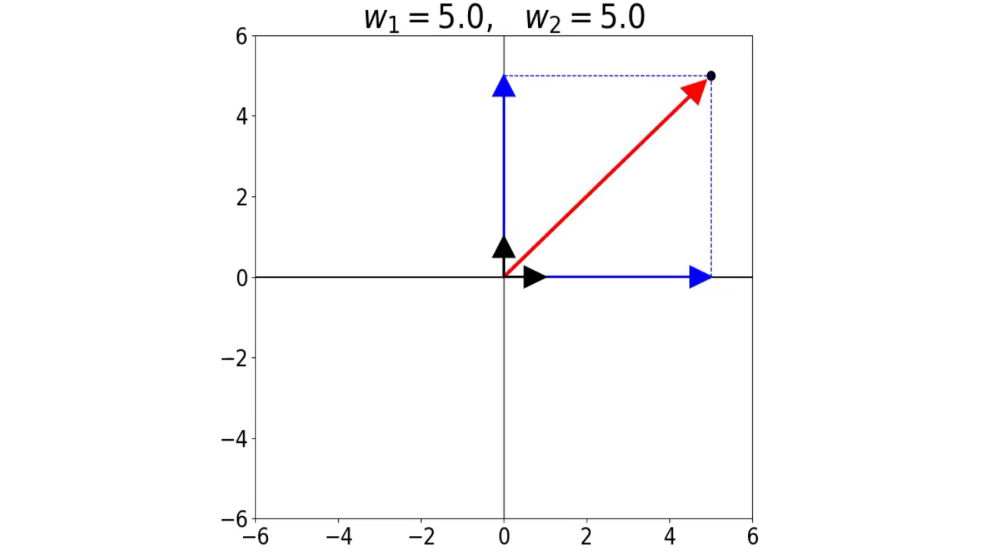
\includegraphics[width=0.5\linewidth]{images/standard_basis.png}
    \caption{Example of a standard basis in $\mathbb{R}^2$.}
    \label{fig:standard_basis}
\end{figure}
\noindent In this case, representing a vector $\displaystyle \mathbf{x}_p$ is a trivial task as the encoding weights will always be given by $\displaystyle \mathbf{w}_p = \mathbf{x}_p$. \newline
It should be noticed that all these properties can also be expressed using the concatenated basis matrix $\displaystyle \mathbf{C}$: knowing that $\displaystyle \mathbf{C}^T\mathbf{C} = \mathbf{CC}^T = \mathbf{I}_{N \times N}$, it is in fact possible to find that
\[\mathbf{w}_p = \mathbf{C}^T\mathbf{x}_p \text{ and } \mathbf{CC}^T\mathbf{x}_p = \mathbf{x}_p \text{ } \forall p \in \{1, \dots, P\}\]
\subsection{Non-standard bases}
When dealing with a non-standard basis, the new vector $\displaystyle \mathbf{w}_p$ acts as the new encoding of $\displaystyle \mathbf{x}_p$ in the transformed feature space whose coordinate axes are defined by the spanning set.
\begin{figure}[H]
    \centering
    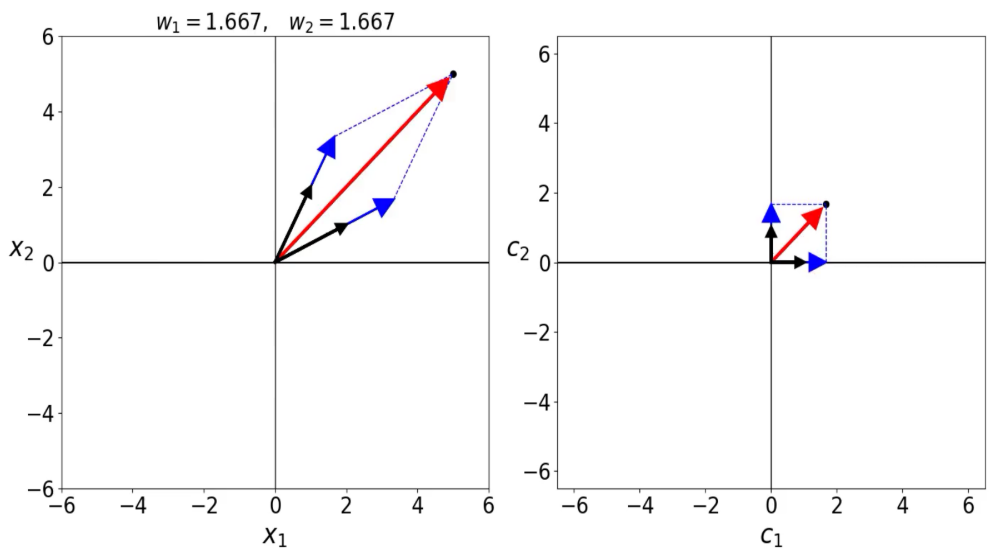
\includegraphics[width=0.5\linewidth]{images/non_standard_basis.png}
    \caption{Example of a non-standard basis in $\mathbb{R}^2$.}
    \label{fig:non_standard_basis}
\end{figure}
\noindent Therefore, using the concatenated basis matrix, the goal is to find the encoding that solves the linear system of equations
\[\mathbf{C}^T\mathbf{Cw}_p = \mathbf{C}^T\mathbf{x}_p \text{ } \forall p \in \{1, \dots, P\} \text{, which is equivalent to solving}\]
\[\min_{\mathbf{w}_1, \dots, \mathbf{w}_P} \frac{1}{P}\sum_{p = 1}^P \lVert \mathbf{Cw}_p - \mathbf{x}_p \rVert_2^2 \text{, which represents the average reconstruction error.}\]
\begin{examplebox}[A non-standard basis in $\displaystyle \mathbb{R}^2$]
    Consider a non-standard basis in $\displaystyle \mathbb{R}^2$ given by
    \[\mathbf{c}_1 = \begin{pmatrix}
        2 \\
        1 \\
    \end{pmatrix} \text{ and } \mathbf{c}_2 = \begin{pmatrix}
        1 \\
        2 \\
    \end{pmatrix}\]
    Expressing a vector using the equation $\displaystyle \mathbf{x}_p = w_{1, p}\mathbf{c}_1 + w_{2, p}\mathbf{c}_2$ reveals that this basis corresponds to a transformation that consists of a rotation followed by a vector shearing.
\end{examplebox}
\section{Vector subspaces}
When representing $\displaystyle N$-dimensional data points $\displaystyle \{\mathbf{x}_p\}_p^P \in \mathbb{R}^N$ using $\displaystyle K \leq N$ basis vectors, the representation incurs in a loss of information because the data points are projected onto a lower-dimensional subspace.
\begin{figure}[H]
    \centering
    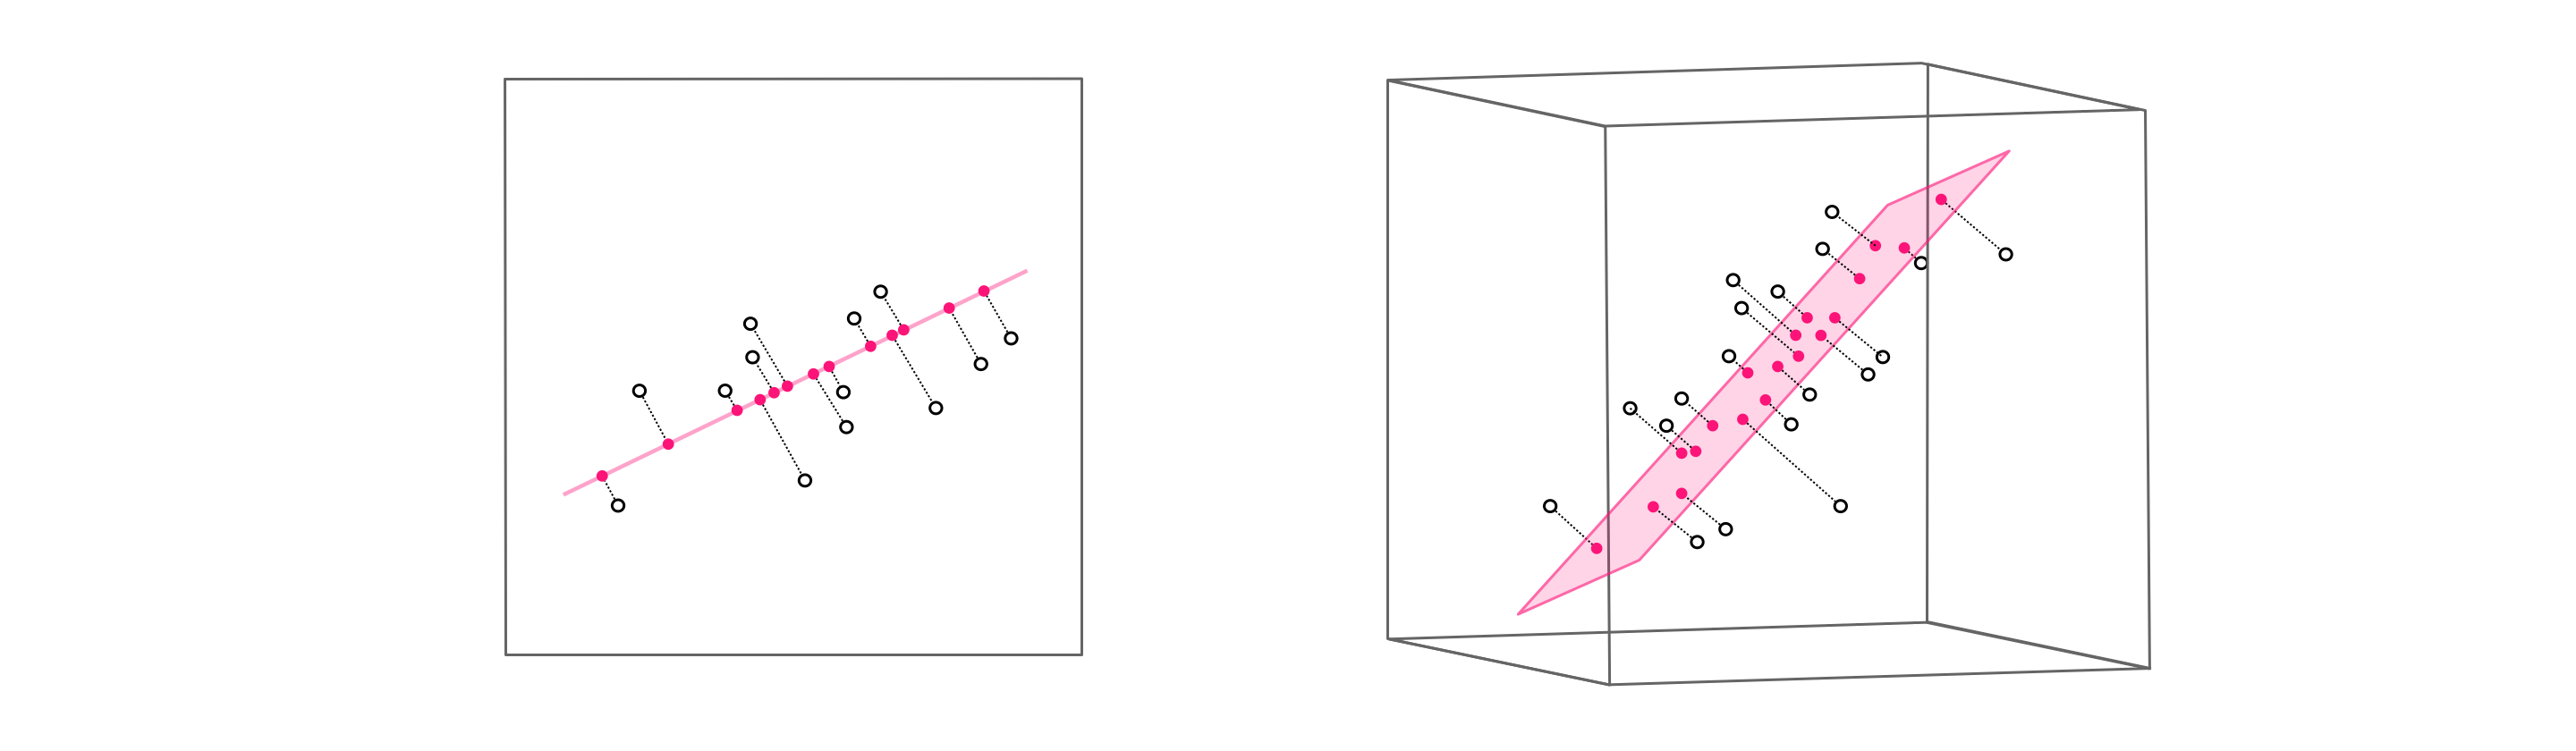
\includegraphics[width=0.5\linewidth]{images/subspace_projections.png}
    \caption{Projecting data points from $\mathbb{R}^3$ onto 1D and 2D subspaces.}
    \label{fig:subspace_projection}
\end{figure}
\noindent In order to minimize the reconstruction error, each data point is projected orthogonally onto the subspace spanned by the basis vectors, meaning that the encoding weights will be computed by solving the linear system of equations
\[\mathbf{C}^T\mathbf{Cw}_p = \mathbf{C}^T\mathbf{x}_p \text{, where $\displaystyle \mathbf{C} \in \mathbb{R}^{N \times K}$.}\]
In fact, this strategy ensures that, during decoding, the projected point provides the best possible approximation of the starting data point within the subspace.
\begin{examplebox}[Projecting a vector from $\displaystyle \mathbb{R}^2$ onto a line]
    Suppose you want to project the vector $\displaystyle \mathbf{x} = (3, 1)^T$ onto the one-dimensional subspace spanned by the basis vector $\displaystyle \mathbf{c} = (1, 1)^T$. \newline
    Since the basis vector is not a unit vector, the encoding weight must be computed as
    \begin{align*}
        \mathbf{c}^T\mathbf{c}w = \mathbf{c}^T\mathbf{x} &\Rightarrow \begin{pmatrix}
            1 & 1 \\
        \end{pmatrix}\begin{pmatrix}
            1 \\
            1 \\
        \end{pmatrix}w = \begin{pmatrix}
            1 & 1 \\
        \end{pmatrix}\begin{pmatrix}
            3 \\
            1 \\
        \end{pmatrix} \\
        &\Rightarrow 2w = 4 \Rightarrow w = 2
    \end{align*}
    Therefore, the reconstructed projection will be given by $\displaystyle w\mathbf{c} = (2, 2)^T$, resulting in a residual reconstruction error of
    \[r = \lVert\mathbf{x} - w\mathbf{c}\rVert_2 = \bigg\lVert \begin{pmatrix}
        3 \\
        1 \\
    \end{pmatrix} - \begin{pmatrix}
        2 \\
        2 \\
    \end{pmatrix}\bigg\rVert_2 = \bigg\lVert\begin{pmatrix}
        1 \\
        -1 \\
    \end{pmatrix}\bigg\rVert_2 = \sqrt{2}\]
\end{examplebox}
\noindent Whenever the chosen basis is orthonormal, the weight encodings can be computed using
\[\mathbf{w}_p = \mathbf{C}^T\mathbf{x}_p \text{ and } \mathbf{CC}^T\mathbf{x}_p \approx \mathbf{x}_p \text{ } \forall p \in \{1, \dots, P\}\]

\chapter{Optimization methods}
\section{The goal of optimization}
Given an objective function $\displaystyle g(\mathbf{w})$, optimization deals with finding the value $\displaystyle \mathbf{w}^*$ that minimizes or maximizes the function, which means that
\[\mathbf{w}^* = \arg\min_{\mathbf{w}} g(\mathbf{w}) \text{ or } \mathbf{w}^* = \arg\max_{\mathbf{w}} g(\mathbf{w})\]
Additionally, maximizing an objective function $\displaystyle g(\mathbf{w})$ is always equivalent to minimizing $\displaystyle -g(\mathbf{w})$.
\subsection{Zero-order optimization}
Since zero-order optimization simply involves analysing the values taken by the objective function, it is possible to distinguish two types of solution:
\begin{itemize}
    \item \textbf{Global optimum: }A point $\displaystyle \mathbf{w}^*$ is a global optimum if it represents a global maximum/minimum among every possible value of $\displaystyle \mathbf{w}$.
    \item \textbf{Local optimum: }A point $\displaystyle \mathbf{w}^*$ is a local optimum if it acts as a local maximum/minimum within some neighbourhood, but not necessarily among every possible value of $\displaystyle \mathbf{w}$.
\end{itemize}
\begin{examplebox}[Zero-order optimization on a sinusoidal function]
    Consider the scalar function $\displaystyle g(w) = \sin(w)$: since this function has period equal to $\displaystyle 2\pi$, it is possible to observe that it has infinitely many global maxima and global minima. \newline
    More specifically the points $\displaystyle w^* = \frac{3\pi}{2} + 2k\pi$, with $\displaystyle k \in \mathbb{Z}$, act as global minima for the function, whereas the points $\displaystyle w^* = \frac{\pi}{2} + 2k\pi$, with $\displaystyle k \in \mathbb{Z}$, act as global maxima for the function.
\end{examplebox}
\subsection{First-order optimization}
First-order optimization involves using (partial) derivatives to find candidate optima by exploiting the fact that, at an extremum of a differentiable function, it is always the case that
\[g'(w^*) = 0 \text{ or, for a multivariate function, } \nabla g(\mathbf{w}^*) = \mathbf{0}_{n \times 1}\]
\begin{examplebox}[First-order optimization on a sinusoidal function]
    Consider the scalar function $\displaystyle g(w) = \sin(w)$: solving $\displaystyle g'(w) = \cos(w) = 0$ reveals that the points $\displaystyle w^* = \frac{\pi}{2} + k\pi$, with $\displaystyle k \in \mathbb{Z}$, act as extrema for the function. \newline
    Using the second derivative $\displaystyle g''(w) = -\sin(w)$ reveals that the points $\displaystyle w^* = \frac{3\pi}{2} + 2k\pi$ act as global minima for the function, whereas the points $\displaystyle w^* = \frac{\pi}{2} + 2k\pi$ act as global maxima for the function.
\end{examplebox}
\section{Hyperplanes}
A hyperplane can be seen as a $\displaystyle N$-dimensional generalization of a line that can be defined as
\[h(\mathbf{w}) = a + \mathbf{b}^T\mathbf{w}\]
Since any point $\displaystyle \mathbf{w}_0$ admits infinitely many direction vectors $\displaystyle \mathbf{d}$, it is possible to find the direction of maximum increase or decrease by evaluating
\[h(\mathbf{w}_0 + \mathbf{d}) = a + \mathbf{b}^T(\mathbf{w}_0 + \mathbf{d}) = a + \mathbf{b}^T\mathbf{w}_0 + \mathbf{b}^T\mathbf{d} \text{, which means that}\]
\[\max_{\mathbf{d}} h(\mathbf{w}_0 + \mathbf{d}) \text{ subject to } \lVert \mathbf{d} \rVert_2^2 = 1 \equiv \max_d \mathbf{b}^T\mathbf{d} = \max_d \lVert \mathbf{b} \rVert_2^2\lVert \mathbf{d} \rVert_2^2 \cos(\theta) \stackrel{\lVert \mathbf{d} \rVert = 1}{=} \max_{\theta} \cos(\theta)\]
Solving this problem reveals that the maximum increase happens whenever $\displaystyle \theta = 0$, which corresponds to the direction vector $\displaystyle \mathbf{d} = \frac{\mathbf{b}}{\lVert \mathbf{b} \rVert_2^2}$, whereas the maximum decrease happens whenever $\displaystyle \theta = \pi$, which corresponds to the direction vector $\displaystyle \mathbf{d} = -\frac{\mathbf{b}}{\lVert \mathbf{b} \rVert_2^2}$.
\section{Local linear approximation}
The gradient of a multivariate function $\displaystyle g(\mathbf{w})$ is a vector $\displaystyle \nabla g(\mathbf{w})$ that contains all the partial derivatives of the function: this vector points towards the direction of maximum ascent, with its magnitude representing the rate of increase in this direction. \newline
Since the gradient vector provides information about ascent and descent, it is possible to approximate the direction of steepest descent of a function $\displaystyle g$ at a point $\displaystyle \mathbf{w}_0$ using the tangent hyperplane
\[g(\mathbf{w}) \approx h(\mathbf{w}) = g(\mathbf{w}_0) + \nabla g(\mathbf{w}_0)^T(\mathbf{w} - \mathbf{w}_0)\]
\begin{figure}[H]
    \centering
    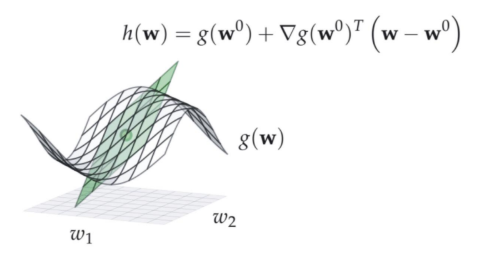
\includegraphics[width=0.3\linewidth]{images/tangent_hyperplane.png}
    \caption{Visualization of the tangent hyperplane of a function.}
    \label{fig:tangent_hyperplane}
\end{figure}
\noindent It should be noticed that, whenever analytical differentiation is not feasible, derivatives can be approximated using the ``central difference'' method used in numerical differentiation, resulting in
\[g'(w_0) = \frac{g(w_0 + \varepsilon) - g(w_0 - \varepsilon)}{2} \text{, for a small $\varepsilon > 0$.}\]
\section{Automatic differentiation}
A computation graph allows to simplify programmatic computations by decomposing a function $\displaystyle g(\mathbf{w})$ into a combination of elementary functions, which are easier to differentiate, and operations.
\begin{figure}[H]
    \centering
    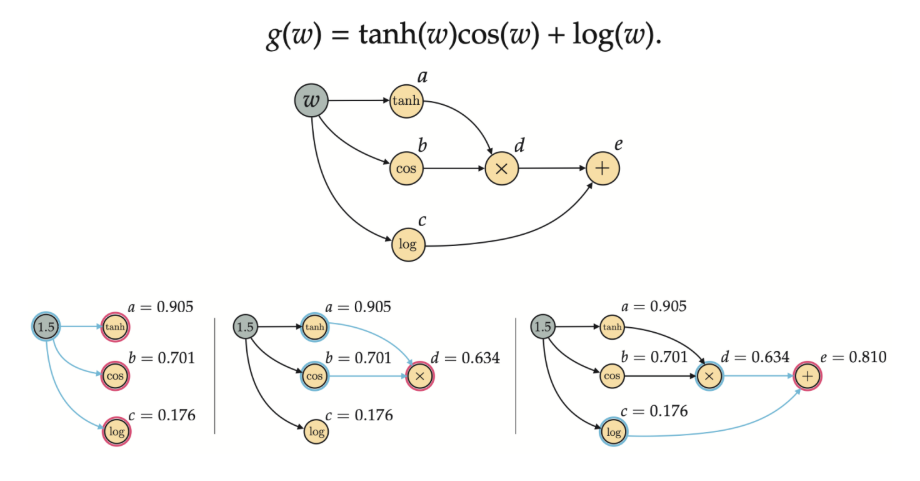
\includegraphics[width=0.35\linewidth]{images/computation_graph.png}
    \caption{A computational graph for the function $\displaystyle g(w) = \tanh(w)\cos(w) + \log(w)$.}
    \label{fig:computation_graph_1}
\end{figure}
\noindent Using ``forward mode'', the graph is traversed left-to-right and each node computes both its value and its gradient with respect to the starting input, providing a simple method for differentiation.
\begin{examplebox}[Running the forward method in a computation graph.]
    Given the function $\displaystyle g(w) = \tanh(w)\cos(w) + \log(w)$, define the following nodes:
    \[a = \tanh(w) \quad b = \cos(w) \quad c = \log(w) \quad d = ab \quad e = c + d\]
    For a starting value $\displaystyle w$, exploit $\displaystyle \frac{dw}{dw} = 1$ to compute the gradient of the child nodes:
    \[\frac{da}{dw} = 1 - \tanh^2(w) \quad \frac{db}{dw} = -\sin(w) \quad \frac{dc}{dw} = \frac{1}{w}\]
    Using this information, it is possible to compute the remaining gradients as well.
    \begin{align*}
        \frac{dd(a, b)}{dw}
            &= \Bigg(\frac{\partial d(a, b)}{\partial a}\frac{da}{dw}\Bigg) + \Bigg(\frac{\partial d(a, b)}{\partial b}\frac{db}{dw}\Bigg) = \frac{da}{dw}b + a\frac{db}{dw} \\
            &= (1 - \tanh^2(w)) - \tanh(w)\sin(w) \\
        \frac{de(d(w), c(w))}{dw}
            &= \Bigg(\frac{\partial e(d(w), c(w))}{\partial d}\frac{dd(w)}{dw}\Bigg)  + \Bigg(\frac{\partial e(d(w), c(w)}{\partial c}\frac{dc(w)}{dw}\Bigg)\\
            &= ((1 - \tanh^2(w))\cos(w) - \tanh(w)\sin(w)) + \frac{1}{w}
    \end{align*}
\end{examplebox}
\noindent The main issue of performing forward mode automatic differentiation lies in the fact that each node computes the gradient with respect to all inputs, leading to massive computational waste when working on large networks. \newline
For this reason, it is more convenient to use ``reverse mode'' automatic differentiation, which consists of a forward pass, where each node uses the input value(s) to compute just the relevant partial derivatives, followed by a backward pass, where gradients are computed by recursively applying the chain rule from the output node.
\begin{figure}[H]
    \centering
    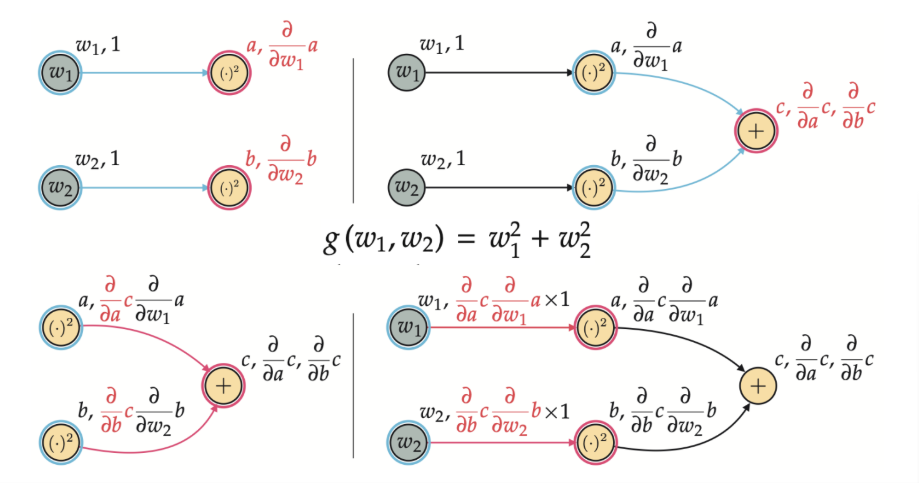
\includegraphics[width=0.35\linewidth]{images/reverse_mode_computation_graph.png}
    \caption{Reverse mode automatic differentiation of the function $\displaystyle g(w_1, w_2) = w_1^2 + w_2^2$.}
    \label{fig:computation_graph_2}
\end{figure}
\noindent Overall, performing reverse mode automatic differentiation allows to significantly reduce computation times, making this strategy useful for developing machine learning models, although memory overhead needs to be considered.
\section{Gradient descent}
Gradient descent exploits the fact that the negative gradient always represents a descent direction to find the global minimum of a function $\displaystyle g(\mathbf{w})$ using the following sequence:
\[\mathbf{w}_k = \mathbf{w}_{k - 1} - \alpha\nabla g(\mathbf{w}_{k - 1})\]
This means that, for an appropriate learning rate $\displaystyle \alpha$, the model uses the current gradient to move towards the direction of steepest descent.
\begin{examplebox}[Optimizing principal component analysis using gradient descent]
    Principal component analysis is an unsupervised learning algorithm that is commonly used to compress high-dimensional data onto a lower-dimensional subspace while retaining data variability in order to preserve information. \newline
    While the algorithm can be optimized by maximizing data variance, one can also apply gradient descent to minimize the loss function, resulting in
    \begin{align*}
        \min_{\mathbf{C}} L(\mathbf{C}) &= \lVert \mathbf{CC}^T\mathbf{X} - \mathbf{X} \rVert_2^2 \text{ subject to } \mathbf{C}^T\mathbf{C} = \mathbf{I} \\
        \nabla_{\mathbf{C}}L(C) &= 2(\mathbf{CC}^T\mathbf{X} - \mathbf{X})\mathbf{X}^T\mathbf{C} \\
        \mathbf{C}_k &= \mathbf{C}_{k - 1} -\alpha\nabla_{\mathbf{C}}L(\mathbf{C}) \text{, with $\mathbf{C}^T\mathbf{C} = \mathbf{I}$.}
    \end{align*}
\end{examplebox}
\noindent While easy to implement, gradient descent is only guaranteed to find a global minimum if $\displaystyle g$ is a convex function as its local minima correspond to the global minima. \newline
In fact, if $\displaystyle g$ is not a convex function, performance depends on the initialization step and learning rate because a small learning rate severely slows down computations, whereas a large learning rate might result in gradient divergence. \newline
For this reason, it can be convenient to monitor gradient descent using a cost function history plot, which plots how the value of a function changes as the algorithm is executed, or by looking at the function's contours.
\begin{examplebox}[Gradient descent on convex and non-convex functions]
    For the convex function $\displaystyle g(w_1, w_2) = w_1^2 + w_2^2 + 2$, the gradient descent algorithm always converges to the global minimum, regardless of the initialization setting.
    \begin{figure}[H]
        \centering
        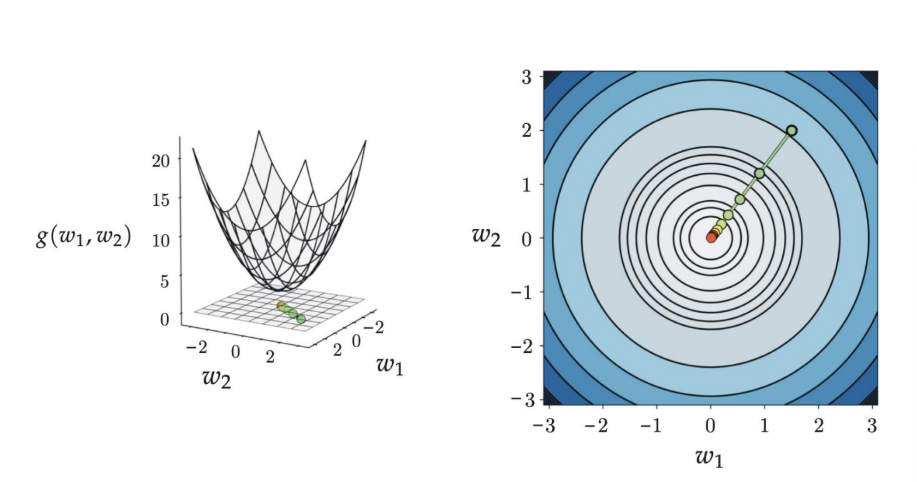
\includegraphics[width=0.4\linewidth]{images/gd_convex.png}
        \caption{Visualization of gradient descent for the function $\displaystyle g(w_1, w_2) = w_1^2 + w_2^2 + 2$.}
        \label{fig:gd_convex}
    \end{figure}
    \noindent By contrast, for the function $\displaystyle g(w) = \sin(3w) + 0.3w^2$, the algorithm's performance does depend on the initialization step because, for instance, choosing $\displaystyle w_0 = -1.5$ allows the algorithm to find a global minimum, whereas starting from $\displaystyle w_0 = 4.5$ causes the algorithm to stop at a local minimum.
    \begin{figure}[H]
        \centering
        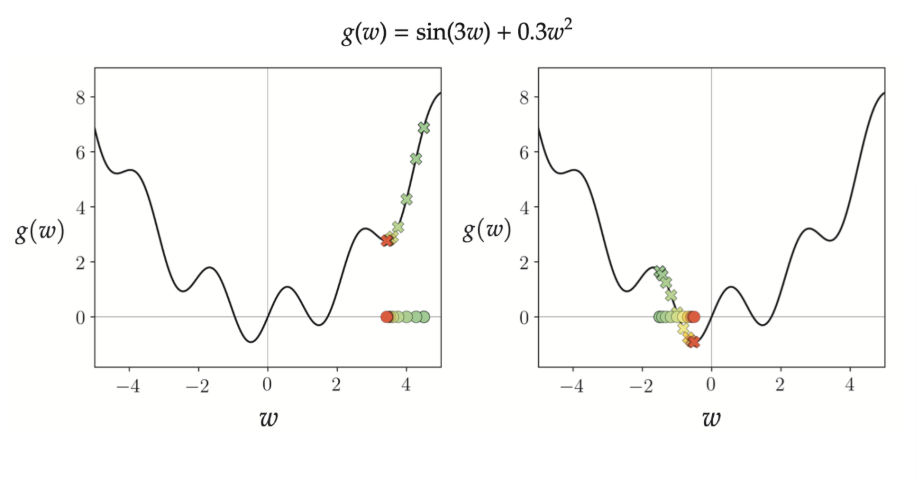
\includegraphics[width=0.4\linewidth]{images/gd_non_convex.png}
        \caption{Visualization of gradient descent for the function $\displaystyle g(w) = \sin(3w) + 0.3w^2$.}
        \label{fig:gd_non_convex}
    \end{figure}
\end{examplebox}
\noindent Overall, it is known that the gradient descent algorithm terminates near the stationary points of a function, where
\[\mathbf{w}_k = \mathbf{w}_{k - 1} - \alpha\nabla g(\mathbf{w}_{k - 1}) \text{ results in } \mathbf{w}_k \approx \mathbf{w}_{k - 1} \Rightarrow \nabla g(\mathbf{w}_{k - 1}) \approx 0\]
For this reason, it is possible to choose the halting criterion among the following options:
\begin{enumerate}
    \item \textbf{Gradient-based criterion: }$\displaystyle \lVert \nabla g(\mathbf{w}_{k - 1}) \rVert_2$ is sufficiently small to suggest that a stationary point has been reached.
    \item \textbf{Step-based criterion: }No significant progress is observed between steps, meaning that, for some small $\displaystyle \varepsilon > 0$, it is the case that
    \[\frac{1}{N}\lVert \mathbf{w}_k - \mathbf{w}_{k - 1} \rVert_2 \leq \varepsilon\]
    \item \textbf{Function value criterion: }The cost function changes negligibly between steps, meaning that, for some small $\displaystyle \varepsilon > 0$, it is the case that
    \[\frac{1}{N}\lVert g(\mathbf{w}_k) - g(\mathbf{w}_{k - 1}) \rVert_2 \leq \varepsilon\]
    \item \textbf{Practical criterion: }The algorithm is terminated after a chosen number of iterations.
\end{enumerate}
\subsection{Zig-zagging gradients}
Whenever the model enters a region where the contours of $\displaystyle g$ are (nearly) parallel, the gradient will start oscillating between steps, causing convergence to slow down.
\subsection{Slow-crawling}
Whenever the model gets close to a stationary point, the gradient descent procedure slows down because the updates are not significant anymore. \newline
This situation becomes problematic whenever $\displaystyle g$ is not a convex function because the algorithm may terminate at a wrong point, such as a local minimum or a saddle point, instead of reaching the global minimum.

\part{Machine Learning}

\chapter{Principal component analysis}
\section{Linear transformations}
Given a matrix $\displaystyle \mathbf{A} \in \mathbb{R}^{m \times n}$, a linear transformation $\displaystyle \mathbf{y} = \mathbf{Ax}$ maps a vector $\displaystyle \mathbf{x} \in \mathbb{R}^n$ to a vector $\displaystyle \mathbf{y} \in \mathbb{R}^m$.
\begin{itemize}
    \item \textbf{Scaling: }If $\displaystyle \mathbf{A}$ is a diagonal matrix, then the transformation $\displaystyle \mathbf{y} = \mathbf{Ax}$ simply stretches or shrinks each axis by the corresponding factor.
    \item \textbf{Rotation: }If $\displaystyle \mathbf{A}$ is an orthonormal matrix, meaning that $\displaystyle \mathbf{A}^T\mathbf{A} = \mathbf{I}$, then the transformation $\displaystyle \mathbf{y} = \mathbf{Ax}$ represents a rotation or a reflection.
    \item \textbf{Shearing: }If $\displaystyle \mathbf{A}$ features some off-diagonal entries, then the transformation $\displaystyle \mathbf{y} = \mathbf{Ax}$ typically results in a slanted vector.
    \item \textbf{Projection: }If $\displaystyle \mathbf{A}$ has rank $\displaystyle k < n$, then the transformation $\displaystyle \mathbf{y} = \mathbf{Ax}$ always results in a loss of information because the vectors collapse into a lower-dimensional space.
\end{itemize}
\section{Learning the projection basis}
Rather than finding the encoding weights for a given basis, principal component analysis aims to learn both the encoding weights $\displaystyle \mathbf{w}_1, \dots, \mathbf{w}_p$ and the basis matrix $\displaystyle \mathbf{C}$ that minimize the mean reconstruction error
\[g(\mathbf{w}_1, \dots, \mathbf{w}_p, \mathbf{C}) = \frac{1}{P}\sum_{p = 1}^P \lVert \mathbf{Cw}_p - \mathbf{x}_p \lVert_2^2 \text{, for a dataset $\{\mathbf{x}_p\}_{p = 1}^P$.}\]
However, if $\displaystyle \mathbf{C}$ is assumed to be orthonormal, it is possible to directly compute $\displaystyle \mathbf{w}_p = \mathbf{C}^T\mathbf{x}_p$ and simplify the objective function to
\[g(\mathbf{C}) = \frac{1}{P}\sum_{p = 1}^P \lVert \mathbf{CC}^T\mathbf{x}_p - \mathbf{x}_p \rVert_2^2\]
\begin{proofbox}
    Assuming $\displaystyle \mathbf{C}$ is orthonormal, meaning that $\displaystyle \mathbf{C}^T\mathbf{C} = \mathbf{I}$, the cost function can be formulated as
    \begin{align*}
        \lVert \mathbf{CC}^T\mathbf{x}_p - \mathbf{x}_p \rVert_2^2
            &= \mathbf{x}_p^T\mathbf{C}^T\mathbf{CCC}^T\mathbf{x}_p -2\mathbf{x}_p^T\mathbf{CC}^T\mathbf{x}_p + \mathbf{x}_p^T\mathbf{x}_p \\
            &\stackrel{\mathbf{C}^T\mathbf{C} = \mathbf{I}}{=} -\mathbf{x}_p^T\mathbf{CC}^T\mathbf{x}_p + \mathbf{x}_p^T\mathbf{x}_p = -\lVert \mathbf{C}^T\mathbf{x}_p \rVert_2^2 + \lVert \mathbf{x}_p \rVert_2^2
    \end{align*}
    Since $\displaystyle \mathbf{x}_p$ is fixed with respect to the optimization over the basis matrix, minimizing the mean reconstruction error is equivalent to maximizing $\displaystyle \lVert \mathbf{C}^T\mathbf{x}_p \rVert$.
\end{proofbox}
\noindent In particular, the assumption that the basis is orthonormal allows to learn each vector independently as the objective function decouples into
\[g(\mathbf{C}) = -\frac{1}{P}\sum_{p = 1}^P\sum_{k = 1}^K (\mathbf{c}_k^T\mathbf{x}_p)^2\]
\section{Optimizing a single basis vector}
Assuming the dataset has been mean-centered and that the basis vector $\displaystyle \mathbf{c}_1$ has unit norm, the quantity
\[h(\mathbf{c}_1) = \frac{1}{P}\sum_{p = 1}^P (\mathbf{c}_1^T\mathbf{x}_p)^2 \text{ represents the sample variance along direction $\mathbf{c}_1$.}\]
By stacking the data points into a matrix $\displaystyle \mathbf{X} = [\mathbf{x}_1, \dots, \mathbf{x}_p] \in \mathbb{R}^{N \times P}$, one can reformulate this quantity as
\[h(\mathbf{c}_1) = \frac{1}{P}\mathbf{c}_1^T\mathbf{XX}^T\mathbf{c}_1 = \mathbf{c}_1^T\Bigg(\frac{1}{P}\mathbf{XX}^T\Bigg)\mathbf{c}_1 = \mathbf{c}_1^T\mathbf{\Sigma c}_1\]
In this setting, $\displaystyle \mathbf{\Sigma}$ is known as the ``empirical covariance matrix'' and, by describing how features vary together, it provides information about the shape of the data cloud through the eigenvectors, which indicate the principal directions in which data spreads the most, and the eigenvalues, which explain the variance along these directions.
\begin{figure}[H]
    \centering
    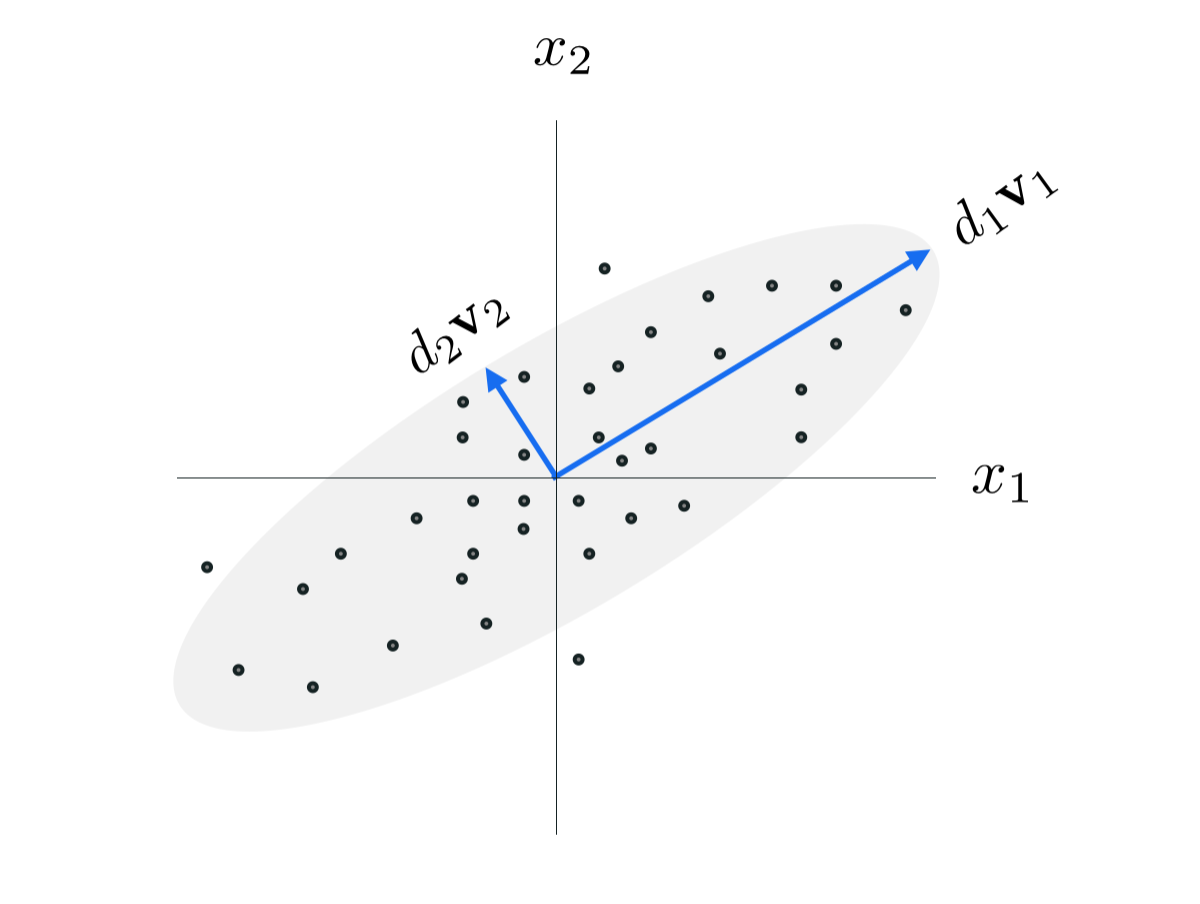
\includegraphics[width=0.25\linewidth]{images/pca_rotation.png}
    \caption{Principal component analysis as a dataset rotation.}
    \label{fig:pca_rotation}
\end{figure}
\noindent Therefore, $\displaystyle h(\mathbf{c}_1)$ will be maximized when $\displaystyle \mathbf{c}_1 = \mathbf{v}_1$ is the eigenvector associated to the largest eigenvalue $\displaystyle \lambda_1$ of the covariance matrix. \newline
More specifically, the scaled eigenvector is known as the ``first principal component'' of the dataset and it explains a proportion of the variance equal to
\[EVR_1 = \frac{\lambda_1}{\sum_{n = 1}^N \lambda_n}\]
\begin{examplebox}[Example of principal component analysis in $\displaystyle \mathbb{R}^2$]
    Consider the following dataset:
    \[\mathbf{x}_1 = \begin{pmatrix}
        2 \\
        1 \\
    \end{pmatrix} \quad\quad \mathbf{x}_2 = \begin{pmatrix}
        0 \\
        0 \\
    \end{pmatrix} \quad\quad \mathbf{x}_3 = \begin{pmatrix}
        1 \\
        -1 \\
    \end{pmatrix}\]
    Start by computing the sample mean $\displaystyle \overline{\mathbf{x}}$ to obtain the mean-centered data points $\displaystyle \mathbf{c}_p = \mathbf{x}_p - \overline{\mathbf{x}}$:
    \[\overline{\mathbf{x}} = \begin{pmatrix}
        1 \\
        0 \\
    \end{pmatrix} \Rightarrow \mathbf{c}_1 = \begin{pmatrix}
        1 \\
        1 \\
    \end{pmatrix} \quad\quad \mathbf{c}_2 = \begin{pmatrix}
        -1 \\
        0 \\
    \end{pmatrix} \quad\quad \mathbf{c}_3 = \begin{pmatrix}
        0 \\
        -1 \\
    \end{pmatrix}\]
    This means that the empirical covariance matrix will be given by
    \[\mathbf{\Sigma} = \frac{1}{3}\sum_{p = 1}^3 \mathbf{c}_p\mathbf{c}_p^T = \begin{pmatrix}
        \frac{2}{3} & \frac{1}{3} \\
        \frac{1}{3} & \frac{2}{3} \\
    \end{pmatrix}\]
    In particular, the eigenvalues of the covariance matrix can be found by solving
    \begin{align*}
        det(\mathbf{\Sigma} - \lambda\mathbf{I})
            &= det\begin{pmatrix}
                \frac{2}{3} - \lambda & \frac{1}{3} \\
                \frac{1}{3} & \frac{2}{3} - \lambda \\
            \end{pmatrix} \\
            &= \Bigg(\frac{2}{3} - \lambda\Bigg)^2 - \frac{1}{9} = \frac{4}{9} - \frac{4\lambda}{3} + \lambda^2 - \frac{1}{9} = \lambda^2 - \frac{4\lambda}{3} + \frac{1}{3} = 0 \\
    \end{align*}
    \[\Delta = \frac{4}{9} > 0 \Rightarrow \lambda_{1, 2} = \frac{\frac{4}{3} \pm \frac{2}{3}}{2} \Rightarrow \lambda_1 = 1, \quad \lambda_2 = \frac{1}{3}\]
    Using these eigenvalues, solving $\displaystyle (\mathbf{\Sigma} - \lambda\mathbf{I})\mathbf{X} = 0$ allows to find the following eigenvectors:
    \begin{align*}
        \mathbf{v}_1
            &= \begin{pmatrix}
                1 \\
                1 \\
            \end{pmatrix} \text{, which corresponds to principal component } \mathbf{v}_1 = \begin{pmatrix}
                \frac{\sqrt{2}}{2} \\
                \frac{\sqrt{2}}{2} \\
            \end{pmatrix} \\
            \mathbf{v}_2 &= \begin{pmatrix}
                1 \\
                -1 \\
            \end{pmatrix} \text{, which corresponds to principal component } \mathbf{v}_2 = \begin{pmatrix}
                \frac{\sqrt{2}}{2} \\
                -\frac{\sqrt{2}}{2} \\
            \end{pmatrix}
    \end{align*}
    In particular, the proportion of data variance explained by the two components will be
    \[EVR_1 = \frac{\lambda_1}{\lambda_1 + \lambda_2} = 0.75 \text{ and } EVR_2 = \frac{\lambda_2}{\lambda_1 + \lambda_2} = 0.25\]
\end{examplebox}
\noindent It should be noticed that the same reasoning can be applied to the other basis vectors when analysing the other principal components.
\subsection{Eigenvalue decompositions}
For a real-valued and symmetric covariance matrix $\mathbf{\Sigma}$, one can compute an orthonormal matrix $\displaystyle \mathbf{V} = [\mathbf{v}_1, \dots, \mathbf{v}_d]$, which is obtained by stacking the eigenvectors of the covariance matrix, and a diagonal matrix $\displaystyle \mathbf{\Lambda}$, which contains the eigenvalues of the covariance matrix, to formulate
\[\mathbf{\Sigma} = \mathbf{V\Lambda V}^T \text{, implying that $\mathbf{\Sigma}$ is always positive semi-definite.}\]
\section{Applications of principal component analysis}
Principal component analysis can be used as an unsupervised learning algorithm that allows to compress high-dimensional data onto a lower-dimensional space, such as a linear manifold, by using the $\displaystyle k << d$ most relevant components to create uncorrelated features that can be exploited to simplify learning tasks or discover data patterns.

\part{Network Science}

\chapter{Understanding networks}
\section{The purpose of network science}
A network is a complex system whose components interact according to three main properties:
\begin{enumerate}
    \item \textbf{Adaptation: }The components of the system mutate and self-organize in order to maintain certain properties.
    \item \textbf{Non-linearity: }A change in the input is not proportional to a change in the output.
    \item \textbf{Emergence: }The system as a whole shows some properties that the individual components do not possess.
\end{enumerate}
\begin{examplebox}[Schelling's segregation model]
    In Schelling's segregation model, agents wish that a fraction $\displaystyle B_a$ of their neighbourhood, which consists of the neighbouring agents, is from the same group. \newline
    At each round, every agent checks the fraction of matching agents $\displaystyle B$ and, if $\displaystyle B < B_a$, it can relocate to a vacant spot, going on until every agent is satisfied.
    \begin{figure}[H]
        \centering
        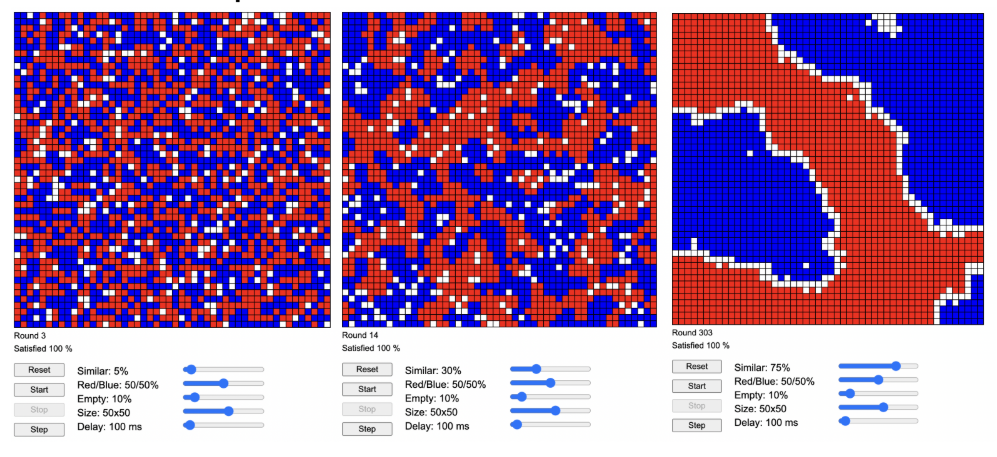
\includegraphics[width=0.5\linewidth]{images/schelling_model.png}
        \caption{Example of Schelling's segregation model.}
        \label{fig:schelling_model}
    \end{figure}
    \noindent In particular, Schelling discovered a threshold $\displaystyle B_{seg}$ such that choosing $\displaystyle B_a < B_{seg}$ leads to a random population configuration, whereas choosing $\displaystyle B_a \ge B_{seg}$ would result in segregation.
\end{examplebox}
\noindent Overall, network science is useful for modelling complex systems by transforming high-dimensional data into feature representations that can be used for inference and pattern discovery.
\section{A formal definition of networks}
A network can be formally represented as a graph $\displaystyle G = (V, E)$ that is described using a set of nodes $\displaystyle V$ and a set of edges $\displaystyle E$ that connect pairs of vertices.
\begin{figure}[H]
    \centering
    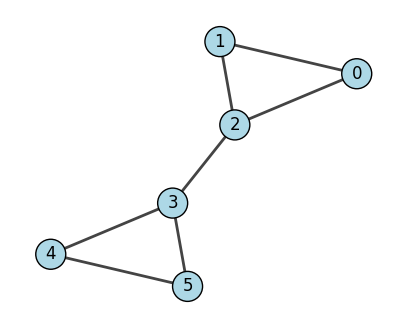
\includegraphics[width=0.25\linewidth]{images/bowtie_graph.png}
    \caption{Example of a graph.}
    \label{fig:bowtie_graph}
\end{figure}
\noindent A graph is said to be ``undirected'' if its edges represent unordered pairs, which means that
\[E = \{\{u, v\}: u, v \in V, u \neq v\} \text{ and } \{u, v\} \in E \Leftrightarrow \{v, u\} \in E\]
By contrast, a graph is said to be ``directed'' if its edges indicate ordered pairs, which means that
\[E = \{(u, v): u, v \in V, u \neq v\} \text{ and } (u, v) \in E \not\Rightarrow (v, u) \in E\]
\subsection{Visualizing a network using an edge list}
A network can be represented using an edge list in which each tuple represents a connection between two endpoints in the graph.
\begin{lstlisting}[
  language=Python,
  captionpos=b,
  caption={Creating a graph from an edge list, which requires $\displaystyle O(|E|)$ memory.},
  label={lst:edge_list}
]
    edges = [(0,1), (0,2), (1,2), (2,3), (3,4), (3,5), (4,5)]
    g_py = ig.Graph(edges=edges, directed=False)
\end{lstlisting}
\noindent Alternatively, a network can be represented as a dataframe in which each row corresponds to an edge and identifies its source and target nodes.
\begin{lstlisting}[
  language=Python,
  captionpos=b,
  caption={Creating a graph from a dataframe.},
  label={lst:df_edge_list}
]
    edge_list_py = pd.DataFrame({
        "source": [0, 0, 1, 2, 3, 3, 4],
        "target": [1, 2, 2, 3, 4, 5, 5]
    })
    g_py = ig.Graph.DataFrame(edge_list_py, directed=False)
\end{lstlisting}
\subsection{Visualizing a network using an adjacency matrix}
It is possible to represent the connections in a network using an adjacency matrix in which $\displaystyle A_{i, j} = 1$ if and only if $\displaystyle (i, j) \in E$ and $\displaystyle A_{ii} = 0 \text{ } \forall i$.
\begin{lstlisting}[
  language=Python,
  captionpos=b,
  caption={Creating a graph from an adjacency matrix, which requires $\displaystyle O(|V|^2)$ memory.},
  label={lst:adjacency_matrix}
]
    adj_matrix = [
        [0, 1, 1, 0, 0, 0],
        [1, 0, 1, 0, 0, 0],
        [1, 1, 0, 1, 0, 0],
        [0, 0, 1, 0, 1, 1],
        [0, 0, 0, 1, 0, 1],
        [0, 0, 0, 1, 1, 0]
    ]
    g_from_matrix = ig.Graph.Adjacency(adj_matrix, mode=ig.ADJ_UNDIRECTED)
\end{lstlisting}
\noindent Additionally, by considering at the definition of an adjacency matrix, it is possible to state that a graph $\displaystyle G = (V, E)$ is undirected if and only if its adjacency matrix is symmetric, meaning that $\displaystyle A^T = A$.
\subsection{Visualizing a network using an adjacency list}
It is possible to summarize the connections in a network using an adjacency list that, for each vertex in the graph, stores a list of its direct neighbours.
\begin{lstlisting}[
  language=Python,
  captionpos=b,
  caption={Representing a graph using an adjacency list, which requires $\displaystyle O(|V| + |E|)$ memory.},
  label={lst:adjacency_list}
]
    adj_list = [
        [1, 2],
        [0, 2],
        [0, 1, 3],
        [2, 4, 5],
        [3, 5],
        [3, 4]
    ]
\end{lstlisting}
\noindent It should be noticed that adjacency lists are not compatible with the \texttt{igraph} library, meaning that a conversion into an edge list or an adjacency matrix is required in order to plot a graph.
\section{Neighbourhoods and subgraphs}
On a graph $\displaystyle G = (V, E)$, an adjacent vertex of a node $\displaystyle v \in V$ is any vertex that is connected to $\displaystyle v$ by an edge in the graph. \newline
In particular, the neighbourhood of a vertex $\displaystyle v$ is a subgraph composed of all the vertices adjacent to $\displaystyle v$, sometimes including $\displaystyle v$ as well, and all the edges connecting these nodes.
\begin{figure}[H]
    \centering
    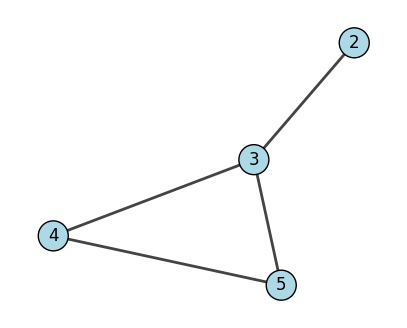
\includegraphics[width=0.25\linewidth]{images/bowtie_graph_neighbourhood.png}
    \caption{Example of a closed neighbourhood within a graph.}
    \label{fig:bowtie_graph_neighbourhood}
\end{figure}
\noindent From a broader perspective, let $\displaystyle G = (V, E)$ be any graph: for a set $\displaystyle S \subseteq V$, the induced subgraph $\displaystyle G[S]$ is a graph whose vertex set is $\displaystyle S$ and whose edge set consists of all the edges with both endpoints in $\displaystyle S$.
\section{Network measures}
Network measures come in handy to describe and investigate the structural properties of a network, such as connectedness or centrality. \newline
For simplicity, it is typically assumed that networks are simple, which means that they contain neither self-loops nor multiple edges connecting the same pair of endpoints.
\begin{figure}[H]
    \centering
    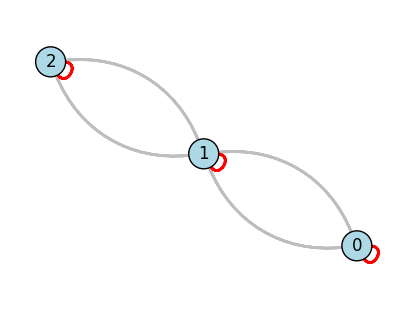
\includegraphics[width=0.25\linewidth]{images/non_simple_graph.png}
    \caption{Example of a graph that is not simple.}
    \label{fig:non_simple_graph}
\end{figure}
\noindent Whenever a network is not simple, the \texttt{simplify} function can be used to turn it into a simple network by removing all redundant elements.
\subsection{Network density}
Network density provides a measure of the number of connections in a graph compared to the maximum possible number of edges. \newline
If $\displaystyle G = (V, E)$ is an undirected graph, its density is given by
\[\delta = \frac{|E|}{|E_{\max}|} = \frac{|E|}{\binom{|V|}{2}} = \frac{2|E|}{|V|(|V| - 1)}\]
On the other hand, if $\displaystyle G = (V, E)$ is a directed graph, its density is defined as
\[\delta = \frac{|E|}{|E_{\max}|} = \frac{|E|}{|V|(|V| - 1)}\]
Overall, real networks tend to be sparse because, even though they consist of many nodes, they feature a very small number of edges that are typically concentrated near some hubs.
\subsection{The degree of a node}
The degree of a node denotes the number of connections that are incident to it.
\begin{itemize}
    \item If $\displaystyle G = (V, E)$ is an undirected graph, the degree of a node is simply defined as
    \[k_i = \sum_j A_{ij} \text{, with } \sum_i k_i = 2|E|\]
    For this reason, the mean degree in an undirected network will be given by
    \[\overline{k} = \frac{1}{|V|}\sum_i k_i = \frac{2|E|}{|V|}\]
    \item If $\displaystyle G = (V, E)$ is a directed graph, it is necessary to make a distinction between a node's in-degree, which denotes the number of incoming connections, and its out-degree, which denotes the number of outgoing connections.
    \begin{align*}
        k_i^{in} &= \sum_j A_{ji} \text{ and } k_i^{out} = \sum_j A_{ij} \text{, with } \sum_i k_i^{in} = \sum_i k_i^{out} = |E| \\
        k_i^{tot} &= k_i^{in} + k_i^{out} \text{, with } \sum_i k_i^{tot} = 2|E|
    \end{align*}
    Therefore, the mean degree in a directed network will be given by
    \[\overline{k^{in}} = \frac{1}{|V|}\sum_i k_i^{in} = \frac{|E|}{|V|} = \frac{1}{|V|}\sum_i k_i^{out} = \overline{k^{out}}\]
\end{itemize}
\section{Weighted networks}
A weighted network is defined as a graph $\displaystyle G = (V, E, w)$, where the function $\displaystyle w: E \to \mathbb{R}^+$ assigns a (positive) weight to each edge in the network.
\begin{figure}[H]
    \centering
    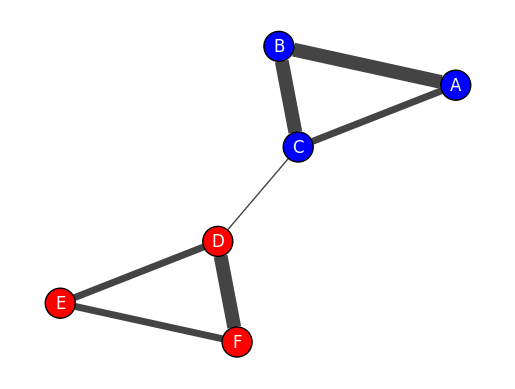
\includegraphics[width=0.25\linewidth]{images/weighted_graph.png}
    \caption{Example of a weighted graph.}
    \label{fig:weighted_bowtie_graph}
\end{figure}
\noindent For this reason, the adjacency matrix of a weighted network can be defined as
\[W_{ij} = \begin{cases}
    w_{ij} &\quad\text{if $(i, j) \in E$} \\
    0 &\quad\text{otherwise} \\
\end{cases}\]
In particular, if a weighted network is undirected, its adjacency matrix is guaranteed to be symmetric, although, if a weighted network is directed, its adjacency matrix may or may not be symmetric.
\subsection{The strength of a node}
The strength of a node can be seen as a generalization of the concept of degree for weighted networks. \newline
In particular, if $\displaystyle G = (V, E, w)$ is an undirected graph, the strength of a node is simply defined as
\[s_i = \sum_j w_{ij}\]
On the other hand, if $\displaystyle G = (V, E, w)$ is a directed graph, it is necessary to make a distinction between a node's in-strength and out-strength.
\[s_i^{in} = \sum_j w_{ji} \text{ and } s_i^{out} = \sum_j w_{ij}\]
\section{The degree distribution of a network}
For an undirected and unweighted graph, the degree distribution describes the frequency of node degrees within the network. \newline
Since this distribution is typically discrete, it can be defined using raw frequencies or by normalizing frequencies into a probability mass function, which describes the probability that a node in the network has a given degree.
\begin{figure}[H]
    \centering
    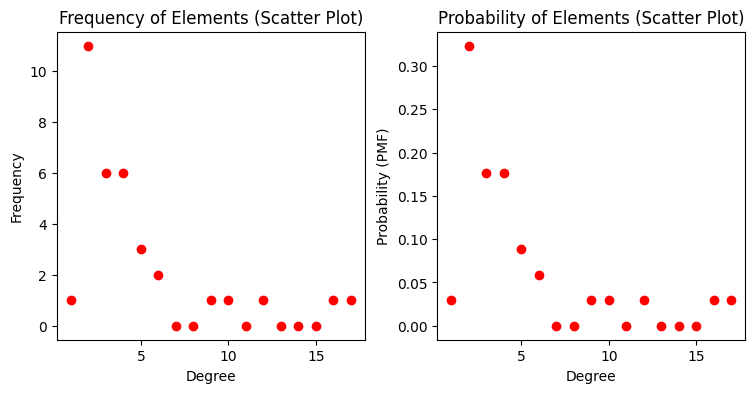
\includegraphics[width=0.45\linewidth]{images/degree_pmf.png}
    \caption{Frequencies and PMF for the degree distribution of the ``Zachary Karate Club'' network.}
    \label{fig:graph_pmf}
\end{figure}
\noindent Alternatively, it is possible to study the degree distribution of a graph through its cumulative distribution function, which denotes the tail probability of the degree distribution.
\begin{figure}[H]
    \centering
    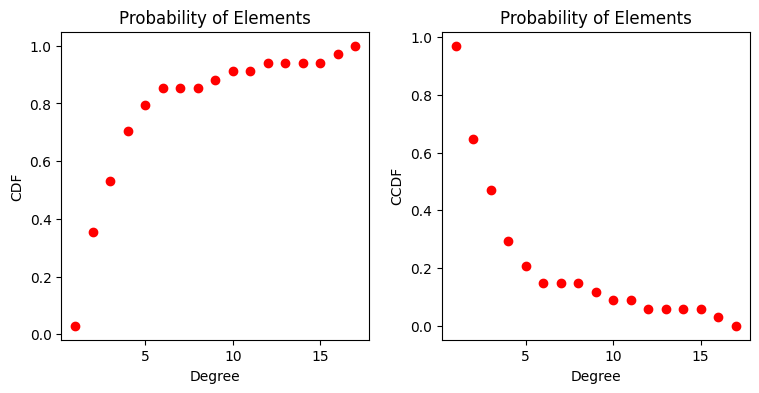
\includegraphics[width=0.45\linewidth]{images/degree_cdf.png}
    \caption{CDF and CCDF for the degree distribution of the ``Zachary Karate Club'' network.}
    \label{fig:graph_cdf}
\end{figure}
\noindent In fact, using the (complementary) cumulative distribution function reveals that many real-world networks follow a power law distribution.

\end{document}